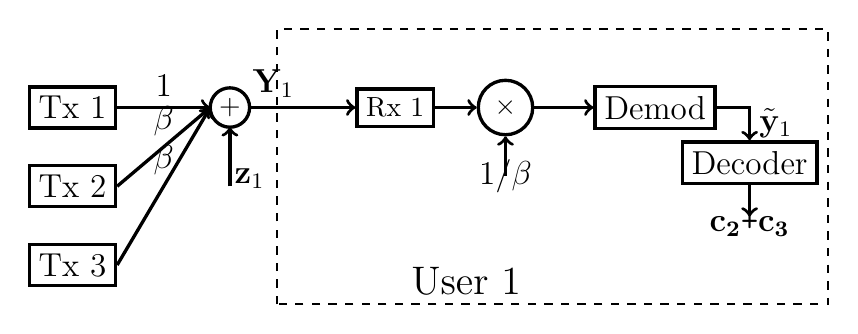
\begin{tikzpicture}

\tikzstyle{block} = [rectangle, draw, very thick, text centered,minimum height=1mm]
\tikzstyle{circleblock} = [circle, draw, very thick, text centered,radius=1mm]

\def \fsize{\large}

%3 Users
\node[block](tx1) at (0,0){\fsize Tx 1};
\node[block](tx2) at (0,-1){\fsize Tx 2};
\node[block](tx3) at (0,-2){\fsize Tx 3};

%Oblique lines to Plus block
\draw[very thick,->] (tx1.east)--(1.75,0)node[draw=none,fill=none,font=\fsize,midway,above]{1};
\draw[very thick,->] (tx2.east)--(1.75,0)node[draw=none,fill=none,font=\fsize,midway,above]{$\beta$};
\draw[very thick,->] (tx3.east)--(1.75,0)node[draw=none,fill=none,font=\fsize,midway,above]{$\beta$};

%From + end to Rx1 end
\draw[black,very thick] (2,0) circle (0.25); \node at (2,0) {+};
\draw [->,very thick] (2,-1) -- (2,-0.25);\node at (2.25,-0.9) {\large $\mathbf{z}_{1}$};

%Receiver 1 block
\node[block](rx1) at (4.1,0){Rx 1}; 
\draw [->,very thick] (2.25,0) -- (rx1.west);
\node[above] at (2.55,0) {\large $\mathbf{Y}_{1}$};

%From Rx1 end to 1/beta multiplicator end
\node[circleblock](mx) at (5.5,0){$\times$};
\draw [<-,very thick] (mx.south)--+(0,-0.5) coordinate (txt2);
\node at (txt2.south) {\large $1/\beta$};

\draw [->,very thick] (rx1.east) -- (mx.west);

%\draw[black,very thick] (4.8,0.4) rectangle (6.2,-0.4); 
%\node[text width=1.2,align=center] at (5.1,0) {\large Subtract $d_{2}\texttt{+}d_{3}$};
%\draw [->,very thick] (4.25,0) -- (4.8,0);

% Input to the Demod
\node[block](demod) at (7.4,0){\fsize Demod};
\draw [->,very thick] (mx.east) -- (demod.west);

%Input to Decoder
\node[block](decoder) at (8.6,-0.7){\fsize Decoder};
\draw [->,very thick](demod.east) --(8.6,0) -- (decoder.north);
\node[right] at (8.6,-0.2) {\large $\tilde{\mathbf{y}}_{1}$};


%Overview dashed rectangle
\draw [->,very thick] (decoder.south) -- +(0,-0.4); 
 \node at (8.6,-1.5){\large $\mathbf{c_{2}}\texttt{+}\mathbf{c_{3}}$};
\draw [dashed,thick] (2.6,-2.5) rectangle (9.6,1);
\node [above] at (5,-2.5) {\Large User 1};

 \end{tikzpicture} 